\documentclass{article}
\usepackage{graphicx}
\usepackage{xcolor}
\usepackage[margin=3cm]{geometry} % margins might need to change in the future check with professor adam 
\setlength{\parindent}{0pt}
\usepackage{pgfgantt}


\begin{document}

\begin{center}
    \Large \textcolor{red}{\textbf{Electronics and Computer Science} \\[0.1cm]} 

    \large \textcolor{red}{Faculty of Engineering and Physical Sciences \\[0.1cm]} 

    \textcolor{red}{University of Southampton \\[1cm]} 

    \vspace{1cm} 

    \textcolor{red}{\textbf{\large Ashwinkrishna Azhagesh} \\[0.5cm]}

    \textbf{14/10/2024} \\[1cm] 

    \textbf{\large An AI Approach to Chaotic Physicl Systems: } \\[1cm]

    \vspace{0.5cm}

    Project supervisor: \textbf{Adam peugeot} \\[0.3cm] 
    Second examiner: \textbf{TBD} \\[1cm]

    Progress report submitted for the award of \\[0.1cm]

    \textbf{\large Bachelors of Science} 
\end{center}

\newpage

{\Huge \textbf{Abstract}}\\[1cm]

Physical laws are generalisation established through empirical observations
of the physical world. It has taken humans centuries to discover, requires huge
amounts of research, repeated experiments and plenty of scientists to produce
an universally accepted law in the scientific community. Thanks to recent
advances in neural networks and increased computational power, we can now
train models to replicate and fasten our discovery of physical laws such as the
laws of motion,also including chaotic systems such as the double pendulum,
drastically shortening the time required to find new physical laws. Furthermore
human’s have a cognitive bias when looking at data, find it difficult to spot
patterns in chaotic systems. This report explores how an AI without any bias or
prior knowledge views the physical world, how it is capable of spotting chaotic
patterns and how it is a tool that can reduce the time taken to make new
discoveries.\\

\newpage

\fbox{\underline{\textbf{Statement of Originality}}}
\\[0.5cm]

- I have read and understood the ECS Academic Integrity information and the University’s
Academic Integrity Guidance for Students.\\

- I am aware that failure to act in accordance with the Regulations Governing Academic Integrity
may lead to the imposition of penalties which, for the most serious cases, may include
termination of programme.\\

- I consent to the University copying and distributing any or all of my work in any form and
using third parties (who may be based outside the EU/EEA) to verify whether my work
contains plagiarised material, and for quality assurance purposes.\\

\fbox{
\underline{\textbf{You must change the statements in the boxes if you do not agree with them.}\\
}}
\\[0.5cm]

We expect you to acknowledge all sources of information (e.g. ideas, algorithms, data) using
citations. You must also put quotation marks around any sections of text that you have copied
without paraphrasing. If any figures or tables have been taken or modified from another source,
you must explain this in the caption and cite the original source.\\

\fbox{
\underline{\textbf{I have acknowledged all sources, and identified any content taken from elsewhere.}\\
}}
\\[0.5cm]

If you have used any code (e.g. open-source code), reference designs, or similar resources that
have been produced by anyone else, you must list them in the box below. In the report, you must
explain what was used and how it relates to the work you have done.\\


\fbox{
\underline{\textbf{I have not used any resources produced by anyone else.}\\
}}
\\[0.5cm]

You can consult with module teaching staff/demonstrators, but you should not show anyone else
your work (this includes uploading your work to publicly-accessible repositories e.g. Github, unless
expressly permitted by the module leader), or help them to do theirs. For individual assignments,
we expect you to work on your own. For group assignments, we expect that you work only with
your allocated group. You must get permission in writing from the module teaching staff before
you seek outside assistance, e.g. a proofreading service, and declare it here.\\

\fbox{
\underline{\textbf{I did all the work myself, or with my allocated group, and have not helped anyone else.}\\
} }
\\[0.5cm]

We expect that you have not fabricated, modified or distorted any data, evidence, references,
experimental results, or other material used or presented in the report. You must clearly describe
your experiments and how the results were obtained, and include all data, source code and/or
designs (either in the report, or submitted as a separate file) so that your results could be
reproduced.\\

\fbox{
\underline{\textbf{The material in the report is genuine, and I have included all my data/code/designs.}\\
}}
\\[0.5cm]

We expect that you have not previously submitted any part of this work for another assessment.
You must get permission in writing from the module teaching staff before re-using any of your
previously submitted work for this assessment.\\

\fbox{
\underline{\textbf{I have not submitted any part of this work for another assessment.}\\
}}
\\[0.5cm]

If your work involved research/studies (including surveys) on human participants, their cells or
data, or on animals, you must have been granted ethical approval before the work was carried
out, and any experiments must have followed these requirements. You must give details of this in
the report, and list the ethical approval reference number(s) in the box below.\\

\fbox{
\underline{\textbf{My work did not involve human participants, their cells or data, or animals.}\\
}}
\\[0.5cm]


ECS Statement of Originality Template, updated August 2018, Alex Weddell aiofficer@ecs.soton.ac.uk\\


\newpage 

\tableofcontents 



\newpage 

\section{Introduction: }

\subsection{Goals: }

It took humans centuries to derivie physical laws, can this process be sped up through AI, by feeding it data and letting the model derive complex laws for us. I aim to derive physical laws, from experimental data. I will explore deriving simpler physical laws such as acceleration without air resistance, and move onto to complex chaotic systems such as pendulums, and explore how an unbiased AI views the physical world, compared to humans who's views of physical systems are naturally biased through systematic learning. 

Can this lead to perhaps different prespectives of viewing the physical world around us, allowing for further progress? 


\subsection{Scope: }


 - Aim to derive simple laws of motions (ie acceleration) through AI frameworks.\\ 

- Move onto more complex systems such as pendulums, and initially explore smaller initial values, moving onto larger initial values, 
thereby increasing the chaos, and difficulty of spotting patterns. \\

- To explore using various AI techniques, (Graph Neural Networks, Deep learning, Neural Networks) in combination with no prior knowledge and observe how and in what form the physical laws are derived.  
- Simulate physical data required using pymunk, and perhaps use real world data from physics labs.\\ 

\section{Literature Review: }

\subsection{ Introduction: }
  
Humans have spent millennia observing the world around us, creating concepts that describe the variables in the physical world, such as mass and force, to derive the laws of motion. In physics, like with all human endevaours, new discoveries and ways of thought are based upon previous works, creating a natural bias in the way we humans approach new problems. All exisiting theories, are therefore somewhat biased, this combined with our pre-existing bias in our biological brains, can introduce some hurdles in our future progress [1,2]. \\

In the 17th Century, Kepler had gotten his hands on the word's most precise data tables on the orbits on planets, using this and his intellect, he spent close to half a decade, and after numerous unsucessful attempts, he had began a scientific revolution at the time, describing Mar's orbit to be an ellipse [3]. In essence, scientists throughout history, much like Kepler, have spent a great deal of time, discovering the right expressions to match the relevent data they have, this at it's core is symbolic regression. Now, a few centuries later, with exponential increases in orders of magnitude in our capability to perform calculations through computers, the process of discovering natural laws and the way to express them, has to some extent resisted automation. \\

One of the core challenges of physics and artificial intelligence, is finding analytical relations automatically, discovering a symbolic expression that accurately matches the data from an unknown function. This problem, due to it's nature, is most certainly NP-hard [4] in principle. The vastness of the space of mathematical constants, further adds to the difficulty. This literature review aims to present the recent advances in deriving expressions and laws through data, how we can avoid human bias by seeking solutions without prior assumptions and describing the various tools and techniques used to achieve this. Then it will introduce the 3-body problem and explore how artificial intelligence is being used to find faster and more efficient solutions.\\ 

\subsection{Symbolic Regression: }

Symbolic regression, is a technique that analyses and searches over the space of traceable mathematical expressions to find the best fit for a data set. By not requiruing prior information about the model, it is unbiased. There are a plethora of various stratergies that have been implemented in solving for various physical laws.\\

There are brute force methods, that leverage the computational power available to \\
brute force\\
some sort of analytical search method- “Distilling Free-Form Natural Laws from Experimental Data\\
narrowing search space through explanable ai - From Kepler to Newton: Explainable AI for Science Discovery\\
various other methods as mentioned here - AI Feynman: a Physics-Inspired Method for Symbolic Regression\\ 
Deep symbolic regression for physics guided by units constraints:
toward the automated discovery of physical laws\\ 


at this point time to move onto more interesting methods: \\

\subsection{Neural Networks: }

NN- Discovering physical concepts with neural networks\\ 

\subsection{ Deep Learning: }
Discovering Symbolic Models from Deep Learning
with Inductive Biases\\ 

Deep Lagrangian Networks:
Using Physics as Model Prior for Deep Learning\\ 

DEEP SYMBOLIC REGRESSION:
RECOVERING MATHEMATICAL EXPRESSIONS FROM
DATA VIA RISK-SEEKING POLICY GRADIENTS\\ 

Maybe talk a bit about the three body problem here: \\ 
\subsection{Transformers: }

SymbolicGPT: A Generative Transformer Model for
Symbolic Regression\\ 

% \subsection{ 4 Body Problem: ?????} too difficult for now 

\subsection{ Conclusion: }


\subsection{Symbolic Regression: }

\subsection{Neural Networks: }

\subsection{Symbolic Neural Networks: }

\subsection{Linear Systems: }

\subsection{Double Pendulum, Chaotic System: }

\section{Progress: }

placeholder 

\section{Project Planning: }

placeholder 

 

\section{ Project Management: }

\subsection{Risk Assessment: }

\begin{center} 
\begin{table}[h]
\centering
\begin{tabular}{|l|l|l|l|l|}
\hline
\textit{Issue}                                                                                                                 & Impact & Prob & Risk & Mitigation                                                                                                                                                                                                             \\ \hline
Unexpected delays and accidents                                                                                                & 3      & 3    & 7    & \begin{tabular}[c]{@{}l@{}}Include contingency plans and a 3 week \\ break between major stages of the project,\\ to allow for unexpected incidents.of the project,\\  to allow for unexpected incidents.\end{tabular} \\ \hline
\begin{tabular}[c]{@{}l@{}}Unable to generate enough \\ experimental data  due to lack\\  of computational power.\end{tabular} & 4      & 1    & 14   & \begin{tabular}[c]{@{}l@{}}Explore alternate more efficient ways of \\ simulating data, consider using cloud\\  infrastructure or potentially the \\ Universities HPC facilities.\end{tabular}                         \\ \hline
\begin{tabular}[c]{@{}l@{}}Challenges learning the double \\ pendulum laws and the derivation.\end{tabular}                    & 2      & 4    & 5    & \begin{tabular}[c]{@{}l@{}}Seek other resources from the Physics Department\\  to learn the Physics required.  Look up \\ explanations online to learn.\end{tabular}                                                   \\ \hline
Interpretability Challenges                                                                                                    & 3      & 2    & 10   & \begin{tabular}[c]{@{}l@{}}Challenges in interpreting how the model\\  works, can be mitigated through visualising\\  the data, plotting results and through\\  seeking ways to explain the model.\end{tabular}        \\ \hline
\end{tabular}
\end{table}
\end{center}


\newpage

\subsection{Project Planning: }

A Gantt chart along with a rough outline of the relevent dates for various submission was made towards the beginning of this project, this alose included contengency planning and short yet frequent breaks every couple weeks.\\ 

blah blah\\ 

\newpage 

\subsection{Gantt Chart: }  


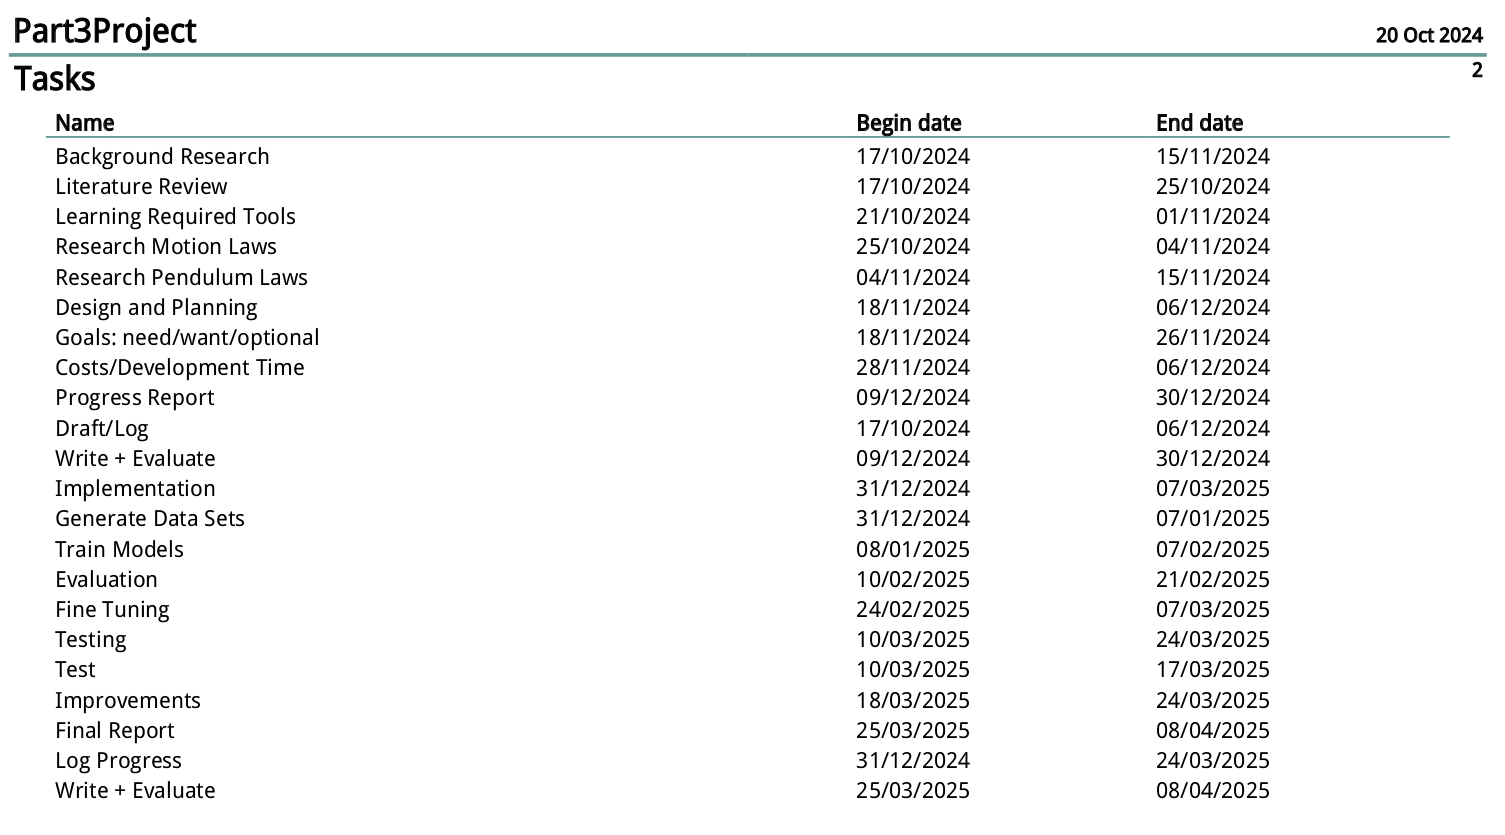
\includegraphics[width=16cm]{Gannt_Chart_Tasks}


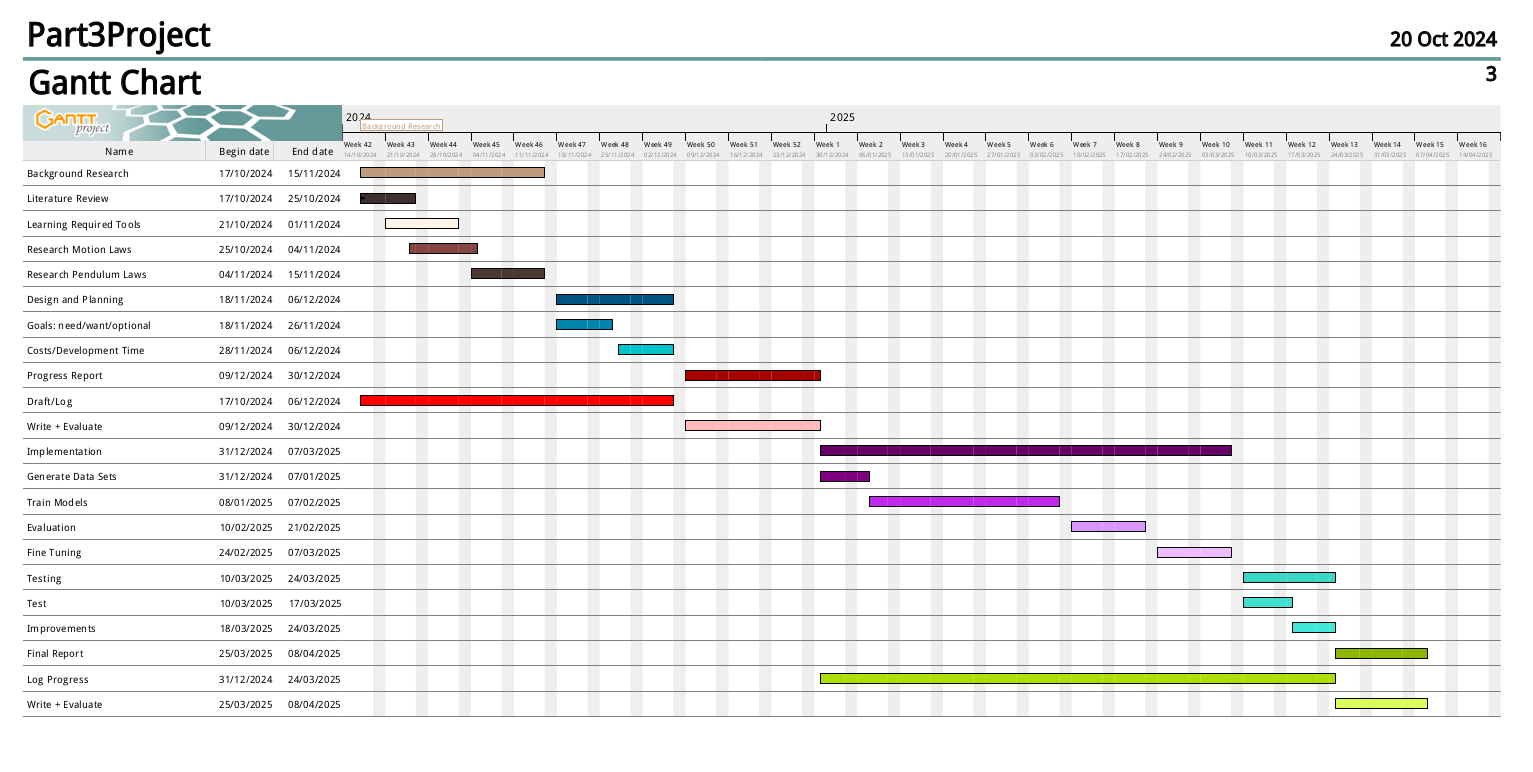
\includegraphics[width=15cm]{Gantt_Chart}

\section{Bibliography: }

[1] C. Wood Powerful ‘Machine Scientists’ Distill the Laws of Physics From Raw Data. Quanta Magazine, 2022.\\ 

[2] M. Schmidt and H. Lipson, Distilling Free-Form Natural Laws from Experimental Data. Science, 324, 5923,
2009.\\

[3] A. Koyr´e, The Astronomical Revolution: Copernicus-
Kepler-Borelli (Routledge, 2013).\\ 

[4] A Computational Inflection for Scientific Discovery by Hope, Tom and Downey, Doug and Weld, Daniel S. and Etzioni, Oren and Horvitz, Eric\\

\end{document}
